\documentclass{article}

%\usepackage{corl_2019} % initial submission
\usepackage[final]{CommMAMT} % Uncomment for the camera-ready ``final'' version
\usepackage{amsfonts}
\usepackage{amsmath}
\usepackage{graphics}
\usepackage{wrapfig}
\usepackage{subcaption}
\usepackage{float} %For minipage - Seems to work well for supplemental - May need to delete
 
\usepackage{epsfig}
\usepackage{lipsum}
\usepackage{todonotes}
\def\UrlFont{\rmfamily}
\usepackage{hyperref}

\DeclareMathOperator*{\argmax}{arg\,max}
\DeclareMathOperator*{\argmin}{arg\,min}

\usepackage{makecell}
\usepackage{color}
\usepackage{amssymb}
\def\UrlFont{\rmfamily}
\usepackage{array,booktabs}
\usepackage{dblfloatfix}
\usepackage{multicol}
\usepackage{tikz}
\usepackage{mathtools}


%\title{Deep Reinforcment Learning with Macro-Actions in Decentralized POMDPs}
%\title{Deep Reinforcment Learning with Macro-Actions in Decentralized Asynchronous Multi-Robot Systems}

%\title{Deep Decentralized Asynchronous Multi-Robot Reinforcment Learning with Macro-Actions under Partial Observability}

\title{Multi-Agent Environments}

% The \author macro works with any number of authors. There are two
% commands used to separate the names and addresses of multiple
% authors: \And and \AND.
%
% Using \And between authors leaves it to LaTeX to determine where to
% break the lines. Using \AND forces a line break at that point. So,
% if LaTeX puts 3 of 4 authors names on the first line, and the last
% on the second line, try using \AND instead of \And before the third
% author name.

% NOTE: authors will be visible only in the camera-ready (ie, when using the option 'final'). 
% 	For the initial submission the authors will be anonymized.

\author{
     \\
}

\makeatletter
\let\thetitle\@title
\let\theauthor\@author

\begin{document}
\maketitle

%===============================================================================

\section{OpenAI Particle Environments}

Each particle environment has a continuous 2D space. The area being shown in the following each picture is under the range: $x\in[-1,1]$, $y\in[-1,1]$. 

\subsection{Cooperative Navigation}

\begin{figure}[h!]
    \centering
    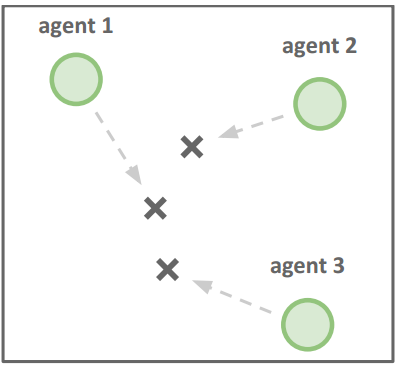
\includegraphics[height=3cm]{spread.png}
\end{figure}

\subsubsection{OpenAI Near-Fully-Observable Settings}

$\bullet$ Goal: 

This task requires three agents to collaboratively cover the three landmarks via physical movements and avoid collision with each other.

$\bullet$ Action space: 

Agent's movement is achieved by receiving a control signal $u=[f_x, f_y]$ including the force applied on the physical body along $x$ axis and $y$ axis. In discrete case, the control signal is discretized into five categories: $[1, 0], [-1, 0], [0,1], [0,-1],[0,0]$. At each time-step, the control signal causes the agents to move towards the force direction in a certain speed $v$, and the resulted travel distance is calculated by $d = v \times dt$, where $dt=0.1$.     

$\bullet$ Observation space: 

Each agent's observation vector includes:

$\,\,\,\,\,\circ$ agent's own speed $[v_x, v_y]$ ;

$\,\,\,\,\,\circ$ agent's own position $[p_x, p_y]$ ;

$\,\,\,\,\,\circ$ landmarks' positions offset $[l_x, l_y]$ ;

$\,\,\,\,\,\circ$ teammates' positions offset $[t_x, t_y]$ .

$\bullet$ Rewards: 

Agents are rewarded based on the minimum agent's distance (a negative value) to each landmark and also penalized for collisions with teammates.

\subsubsection{Partially-Observable Settings}

There are two options for modifying this environment to be partially observable.

$\bullet$ Option 1: 

Add a observation radius $(r=1)$ to each agent. This particular partially observable Cooperative Navigation domain was introduced in the paper \href{http://aaai-rlg.mlanctot.info/papers/AAAI20-RLG_paper_15.pdf}{Decentralized Multi-Agent Actor-Critic with Generative Inference}.

$\bullet$ Option 2:

Introduce observation flickering such that:

$\,\,\,\,\,\circ$ agent's own speed $[v_x, v_y]$ (fully-observable);

$\,\,\,\,\,\circ$ agent's own position $[p_x, p_y]$ (fully-observable);

$\,\,\,\,\,\circ$ landmarks' positions offset $[l_x, l_y]$ (flickering $P_f=0.3$);

$\,\,\,\,\,\circ$ teammates' positions offset $[t_x, t_y]$ (flickering $P_f=0.3$).

\subsection{Cooperative Predator-Prey}

\begin{figure}[h!]
    \centering
    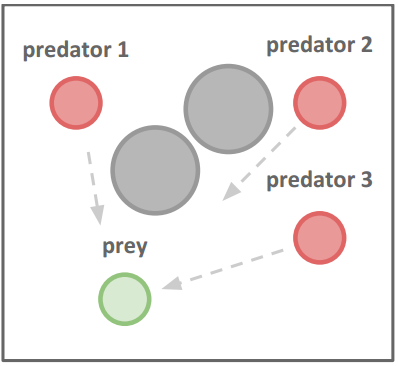
\includegraphics[height=3.5cm]{tag.png}
\end{figure}

\subsubsection{OpenAI Near-Fully-Observable Settings}

$\bullet$ Goal:  

Three slower predators is tasked with capturing a faster prey around a randomly generated environment with two large landmarks impeding the way. Originally, this is a competitive domain, while we impose a hard-coded policy to the prey in order to make this task fully cooperative. We designed two alternative polices to the prey: 

$\,\,\,\,\,A:$ moves towards the sampled positions with the largest distance to all the predators;

$\,\,\,\,\,B:$ moves towards the sampled positions with the largest distance to the closest predator;

The predators are allowed to move around in the entire continuous space, while the prey's movement are bounded in the ares shown in the picture.

$\bullet$ Action space: 

Same as the one mentioned above.

$\bullet$ Observation space: 

Each agent's observation vector includes:

$\,\,\,\,\,\circ$ agent's own speed $[v_x, v_y]$ ;

$\,\,\,\,\,\circ$ agent's own position $[p_x, p_y]$ ;

$\,\,\,\,\,\circ$ landmarks' positions offset $[l_x, l_y]$ ;

$\,\,\,\,\,\circ$ teammates' positions offset $[t_x, t_y]$ ;

$\,\,\,\,\,\circ$ prey's position offset $[\text{prey}_{p_x}, \text{prey}_{p_y}]$ ;

$\,\,\,\,\,\circ$ prey's speed $[\text{prey}_{v_x}, \text{prey}_{v_y}]$ .

$\bullet$ Rewards: 

Agents are rewarded $+10$ if and only if any predator collides with the prey.

\subsubsection{Partially Observable Settings}

Here, we have two options for modifying this environment to be partially observable.

$\bullet$ Option 1: 

Add a observation radius $(r=1)$ to each agent. This particular partially observable Predator-Prey domain was introduced in the paper \href{http://aaai-rlg.mlanctot.info/papers/AAAI20-RLG_paper_15.pdf}{COMIX}.

$\bullet$ Option 2:

Introduce observation flickering such that:

$\,\,\,\,\,\circ$ agent's own speed $[v_x, v_y]$ ;

$\,\,\,\,\,\circ$ agent's own position $[p_x, p_y]$ ;

$\,\,\,\,\,\circ$ landmarks' positions offset $[l_x, l_y]$ (flickering $P_f=0.3$) ;

$\,\,\,\,\,\circ$ teammates' positions offset $[t_x, t_y]$ (flickering $P_f=0.3$) ;

$\,\,\,\,\,\circ$ prey's position offset $[\text{prey}_{p_x}, \text{prey}_{p_y}]$ (flickering $P_f=0.3$) ;

$\,\,\,\,\,\circ$ prey's speed $[\text{prey}_{v_x}, \text{prey}_{v_y}]$ (flickering $P_f=0.3$).

{\color{red} Q: Regarding the two options on changing the above domains to be partially observable, which one makes more sense?}


\subsection{Speaker and Listener}

\begin{figure}[h!]
    \centering
    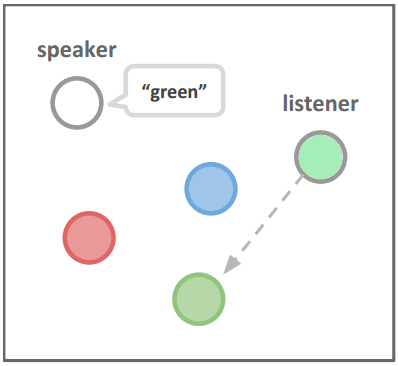
\includegraphics[height=3.5cm]{sp_lis.png}
\end{figure}

\subsubsection{OpenAI Near-Fully-Observable Settings}

$\bullet$ Goal:

This domain involves two agents: a speaker (not moveable) and a listener (moveable). The listener must navigate to a target landmark which is only observable to the speaker, but the listener is allowed to observe the message broadcast by the speaker at each time-step. Therefore, the speaker has to learn to produce the correct message indicating the correct target to the listener.    

$\bullet$ Action Space:

$\,\,\,\,\,\circ$ the speaker has three discrete communicating actions;

$\,\,\,\,\,\circ$ the listener only performs moving actions as mentioned above.

$\bullet$ Observation Space:

$\,\,\,\,\,\circ$ the speaker observes the target landmark color: red ($[0.75, 0.25, 0.25]$), green ($[0.25, 0.75, 0.25]$) or blue ($[0.25, 0.25, 0.75]$);

$\,\,\,\,\,\circ$ the listener observes:

$\,\,\,\,\,\,\,\,\,\,\diamond$ agent's own speed $[v_x, v_y]$ ;

$\,\,\,\,\,\,\,\,\,\,\diamond$ landmarks' positions offset $[l_x, l_y]$ ;

$\,\,\,\,\,\,\,\,\,\,\diamond$ teammate's message, a one-hot vector indicates the target landmark interpreted from the speaker's communicating action.

$\bullet$ Rewards:

At each time-step, agents receive a negative reward respect to the distance between the listener to the correct landmark.

\subsubsection{Partially Observable Settings}

Here, we can also have two options for modifying this environment to be partially observable.

$\bullet$ Option 1: 

Add a observation radius $(r=1)$ to each agent.

{\color{red} Q: How to implement this observation range, limiting the observation on landmarks, limiting the observation on speaker's message, or both?}

{\color{red} Q: Whether the resulting domain still makes sense or not?}

$\bullet$ Option 2:

Introduce observation flickering.

{\color{red} Q: Which part of the observation to be flickering: the observation on landmarks, the observation on speaker's message, or both?}

\subsection{Simultaneous Speaker and Listener}

\begin{figure}[h!]
    \centering
    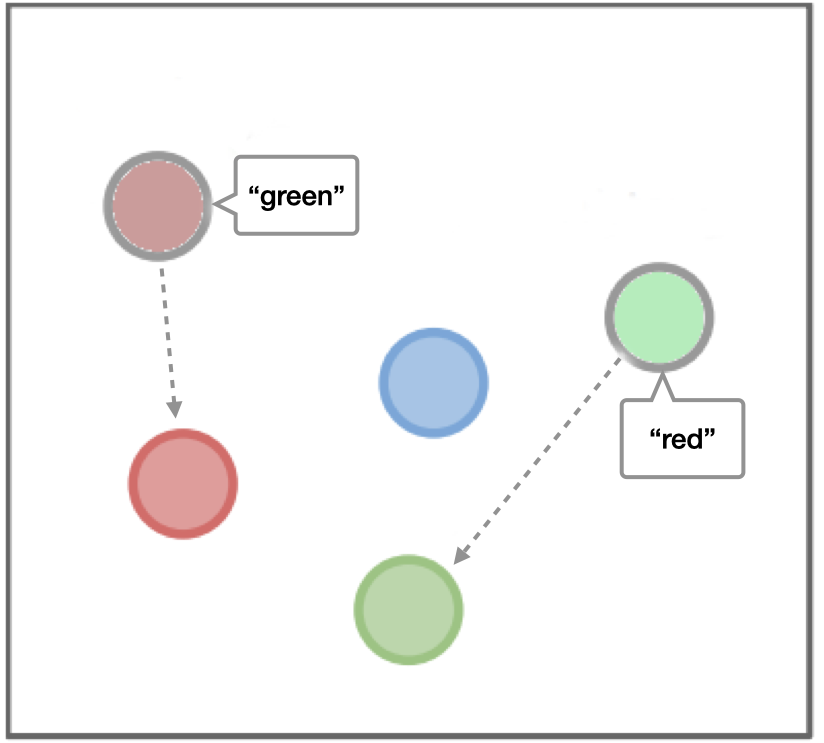
\includegraphics[height=3.5cm]{ref.png}
\end{figure}

\subsubsection{OpenAI Near-Fully-Observable Settings}

This domain is very similar to the speaker and listener problem where both agents are simultaneous speaker and listener. Each agent has to learn to communicate the correct target landmark with the partner, and navigate to its own target landmark. The action space, observation space and rewards are same as mentioned in speaker and listener domain. 

\subsubsection{Partially Observable Settings}

{\color{red} Q: same questions as above.}

\newpage
\section{Communicable Multi-Agent Multi-Target Domain (CommMAMT)}

\begin{figure}[h!]
    \centering
    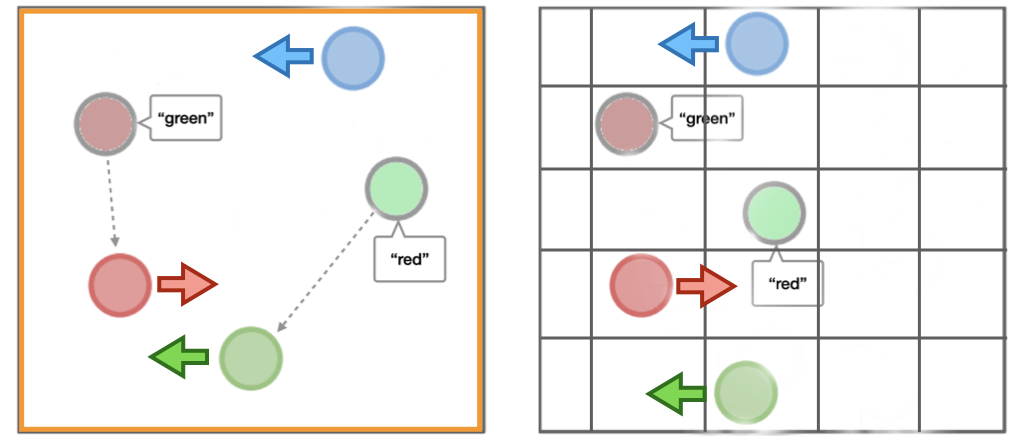
\includegraphics[height=5cm]{commMAMT.png}
\end{figure}

This task consists of two agents and three moving targets (with different colors) operating in a continuous bounded world (\textbf{left}) or a toroidal grid world (\textbf{right}). At each episode, the positions of the two agents and the three targets are randomly initialized. 

In the continuous environment, each target moves horizontally in a constant speed, while each agent moves in the same way as mentioned in the above particle environments. Note that, both agents and targets will be rebounded when they touch the boundaries. 

In the toroidal grid world, each agent has four moving actions: \emph{up}, \emph{down}, \emph{right}, \emph{left} and a \emph{stay} action executed with a transition noisy (0.1), and the each target still moves in the horizontal manner. 

In both cases, each agent always observers its own location or speed, and it is always allowed to receive the message from teammate, but only sometimes observes the each landmark's positions. 

Each agent's correct target is only known by the partner. Therefore, agents have to learn to communicate the correct target landmark with the partner, and navigate to its own target landmark. 

$\bullet$ Observation Space:

\begin{table*}[h]
    \caption {Observation Space}
    \label{obs space}
    \centering
    \begin{tabular}{l|r}
    \toprule
        Continuous World & Grid World \\
        \cmidrule(lr){1-2}
        partner's target's color & partner's target's color\\
        agent's own speed & agent's own position\\
        landmarks' positions offset (flickering) & landmarks' positions (flickering)\\
        partner's message ({\color{red} flickering?}) & partner's message ({\color{red} flickering?})\\
    \bottomrule
    \end{tabular} 
\end{table*}

$\bullet$ Rewards:

\begin{table*}[h]
    \caption {Rewards}
    \label{obs space}
    \centering
    \begin{tabular}{p{4cm}|p{3cm}}
    \toprule
        Continuous World & Grid World \\
        \cmidrule(lr){1-2}
        At each time-step, agents receive a negative reward respect to summation of the distance between each agent to the corresponding correct landmark.
& Only a terminal reward is issued when two agents capture the correct targets simultaneously.\\
    \bottomrule
    \end{tabular} 
\end{table*}


\newpage
$\bullet$ Action Space:

\begin{table*}[h]
    \caption {Moving Actions}
    \label{moving actions}
    \centering
    \begin{tabular}{l|r}
    \toprule
        Continuous World & Grid World \\
        \cmidrule(lr){1-2}
        $u=[0,1]$ & up\\
        $u=[0,-1]$ & down\\
        $u=[-1,0]$ & left\\
        $u=[1,0]$ & right\\
        $u=[0,0]$ & stay\\
    \bottomrule
    \end{tabular} 
\end{table*}

$\,\,\,\,\,\circ$ Communicating actions:

$\,\,\,\,\,\,\,\,\,\,\diamond$ Option 1, pre-defined three discrete communicating actions indicate the correct target:

\begin{figure}[h!]
    \centering
    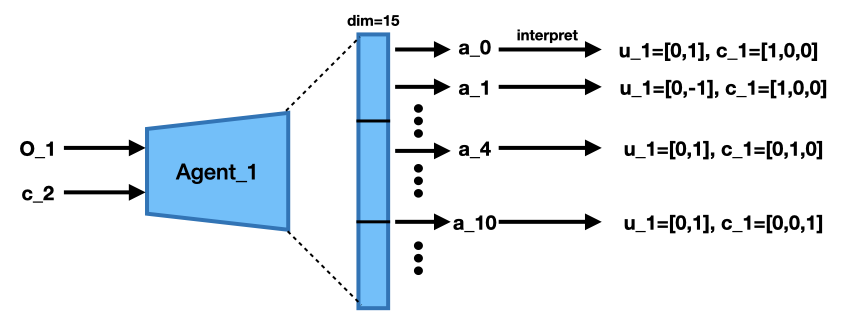
\includegraphics[height=3.5cm]{discrete_c.png}
\end{figure}

$\,\,\,\,\,\,\,\,\,\,$ Agent needs to learn \textbf{which} message to send.

$\,\,\,\,\,\,\,\,\,\,\diamond$ Option 2, no pre-defined communicating action.

\begin{figure}[h!]
    \centering
    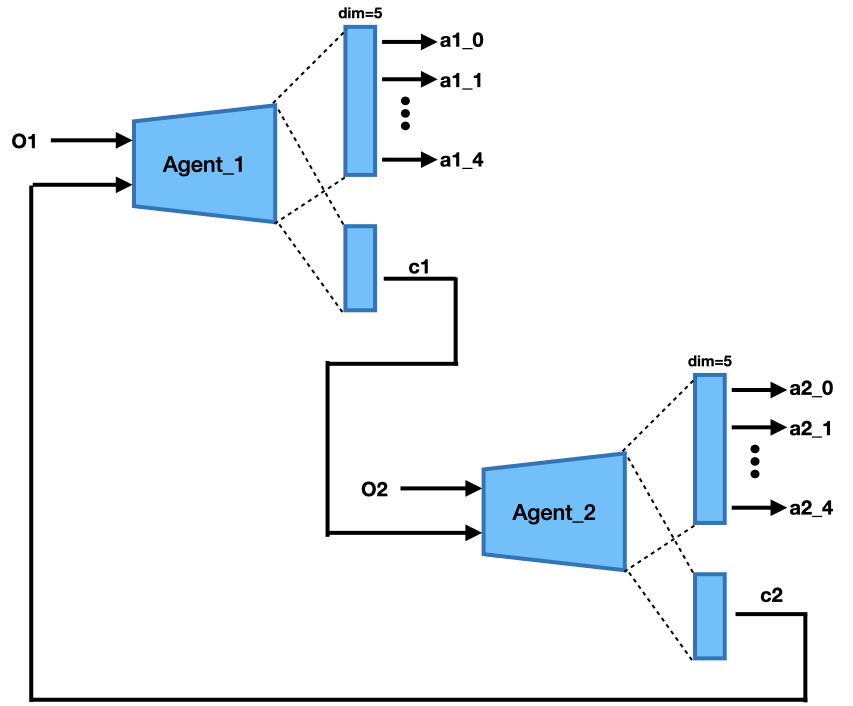
\includegraphics[height=7cm]{luke_c.png}
\end{figure}

$\,\,\,\,\,\,\,\,\,\,$ Agent needs to learn \textbf{what} message to send.




\end{document}
